\begin{table}[htbp]
\begin{center}
\caption{Summary of training datasets.}
\begin{tabular}{ c|c|c|c } 
 \hline
 Datasets &  Data & Features & Non-zeros \\ 
 \hline
  ijcnn & 35,000 & 22 &  455,000\\
  covtype & 581,012 & 54 & 7,521,450\\ 
 %w8a & 49,749  & 300 & 2 \\ 
 real-sim &  72,309 & 20,958 &  3,709,083 \\
 rcv1 & 20,242 & 47,236 &  50,233,657\\
%  \hline
% SUSY & 5,000,000 & 18 &  88,938,127 \\
 %epsilon &  400,000 & 2,000 &  800,000,000 \\
 %kdd12 & 119,705,032 & 54,686,452 & 0 \\
 \hline
\end{tabular}
\label{metadata}
\end{center}
\end{table}

\begin{figure*}[htbp]
\subfigure[speedup on ijcnn]{
\centering
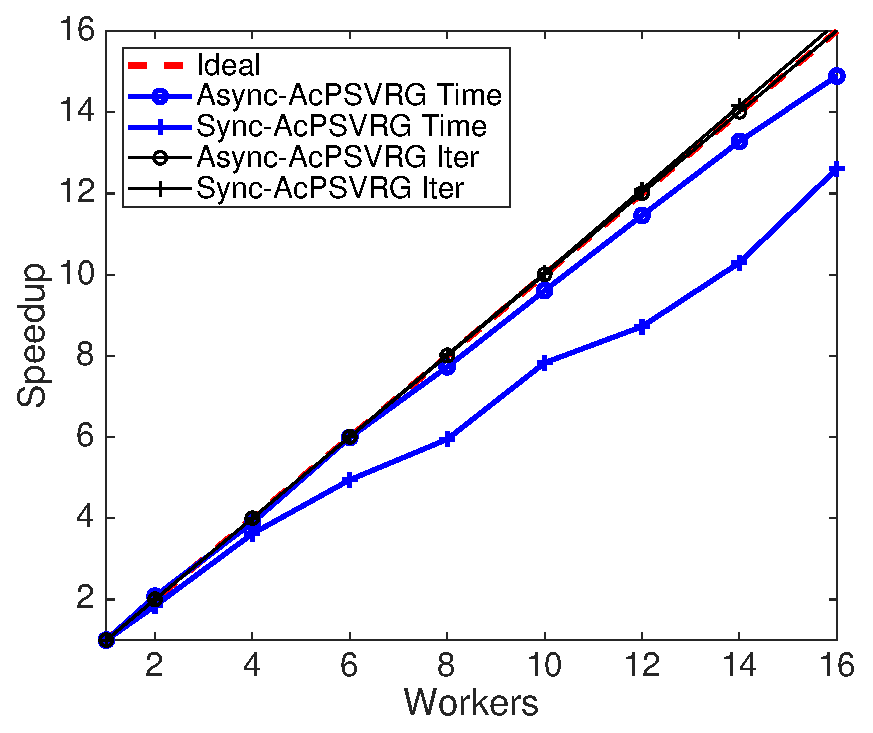
\includegraphics[width=0.24\linewidth]{Figures/ijcnn_speedup_FSVRG.eps}}%
\subfigure[speedup on covtype]{
\centering
\includegraphics[width=0.24\linewidth]{Figures/covtype_speedup_FSVRG.eps}}%
\subfigure[speedup on real-sim]{
\centering
\includegraphics[width=0.24\linewidth]{Figures/real-sim_speedup_FSVRG.eps}}%
\subfigure[speedup on rcv1]{
\centering
\includegraphics[width=0.24\linewidth]{Figures/rcv1_speedup_FSVRG.eps}}%
\setlength{\abovecaptionskip}{2pt}
\caption{Scalability analysis of Sync-AcPSVRG and Async-AcPSVRG with iteration and time speedup. }
\label{fig:FSVRG_speedup}
\end{figure*}

We present our empirical results in this section. For our experiments, we study logistic regression loss function with $L_2$ regularization. The problem can be formulated as optimization problem \eqref{problem} with $f_i(x) = \log(1+e^{-y_iz^T_i{x}})$, $h(x) = \frac{\tau}{2}\|{x}\|^2$, where $z_i\in\R^d$ and $y_i$ is the corresponding label for each $i$. Further, the $L_2$ regularization weight $\tau$ is set $10^{-4}$ in all experiments. We evaluate the following state-of-the-art variance reduction algorithms for our experiments: 1) SVRG \cite{Johnson12}, 2) ProxASAGA\cite{pedregosa2017breaking} and 3) Katyusha \cite{Allen-Zhu17}. The learning rates are tuned for these algorithms in our experiments, and the results shown in this section are based on the best learning rate for each algorithm we achieved.


All the algorithms were implemented in C++ and OpenMPI{\footnote{All simulations were performed on Amazon EC2 t2.large instances with 8 GB RAM.}}. We run our experiments on datasets from LIBSVM website{\footnote{https://www.csie.ntu.edu.tw/~cjlin/libsvmtools/datasets/binary.html}}, as shown in Table \ref{metadata} . The epoch size $m_1$ initially is chosen as 125 in all our experiments and it grows in each epoch by a constant of $\gamma$ = 1.5. In AcPSVRG, we set step sizes $\eta$ and $\beta_s$ to satisfy our assumptions in lemmas and theorems with $\tau\sim P$, where $P$ is the number of workers.

In the first experiment, we compare the speedup achieved by our synchronous and asynchronous algorithm. To this
end, for each dataset we first measure the time required for the algorithm to reach the accuracy of $10^{-10}$. The iteration speedup with $P$ processes is defined as 
\[
 \text{iteration speedup} = \frac{\text{number of iterations with single worker}}{\text{avg. number of iterations with $P$ workers}} \]
and the time speedup is defined as 
 \[
  \text{time speedup} = \frac{\text{runtime with single worker}}{\text{runtime with $P$ workers}}.
\]
%\begin{figure}[htbp]
%\centerline{\includegraphics{fig1.png}}
%\caption{Example of a figure caption.}
%\label{fig}
%\end{figure}


Results in Figure \eqref{fig:FSVRG_speedup} show the speedup on various datasets. As shown by Figure \eqref{fig:FSVRG_speedup}, we achieve remarkable speedups for all the datasets. Both synchronous and asynchronous versions show linear iteration speedup in all data sets. Furthermore, the highest
time speedup for Async-AcPSVRG is achieved for ijcnn dataset which has the fewest number of features compared to other datasets we considered in this experiment. Evidently, the time speedup achieved by Async-AcPSVRG is higher than ones obtained by Sync-AcPSVRG. The speedup for Sync-AcPSVRG improves with the size of datasets, since the synchronization cost, which includes both communication time and waiting time, is dominant compared to computation time on small datasets. The results for Async-AcPSVRG show better scalability compared with \cite{Reddi2015,Meng2016}.


\begin{figure*}[htbp]
\subfigure[comparison on ijcnn]{
\centering
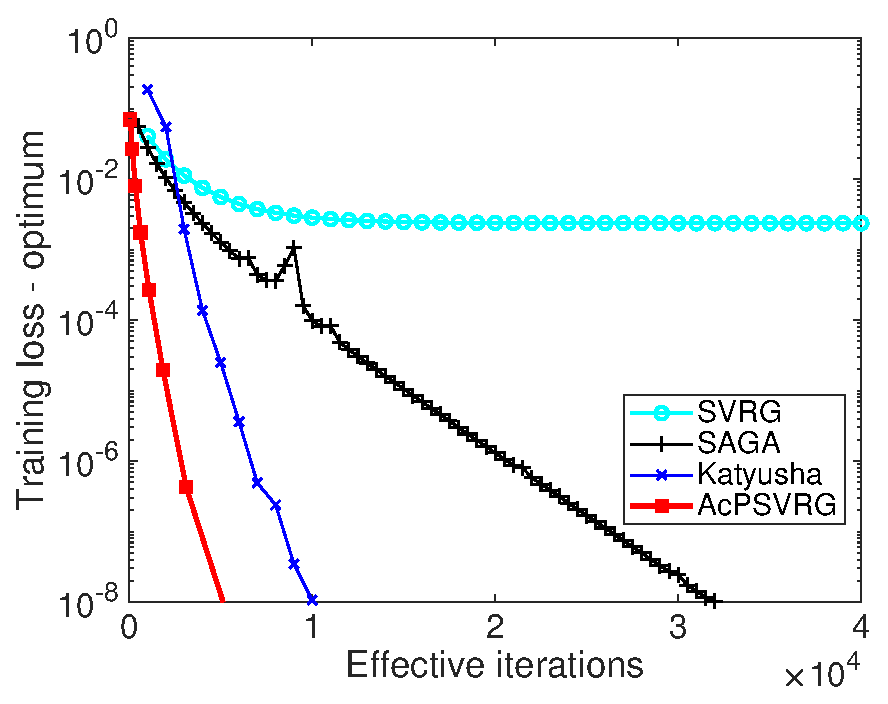
\includegraphics[width=0.24\linewidth]{Figures/ijcnn_obj_dev_comparison_1worker.eps}}%
\subfigure[{comparison on covtype}]{
\centering
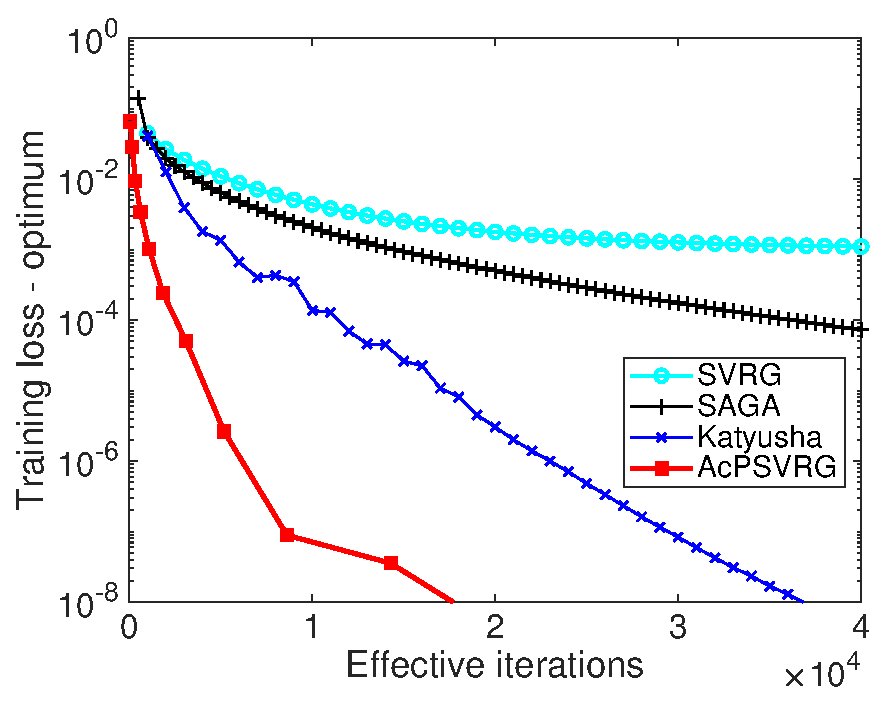
\includegraphics[width=0.24\linewidth]{Figures/covtype_obj_dev_comparison_1worker.eps}}%
\subfigure[comparison on real-sim]{
\centering
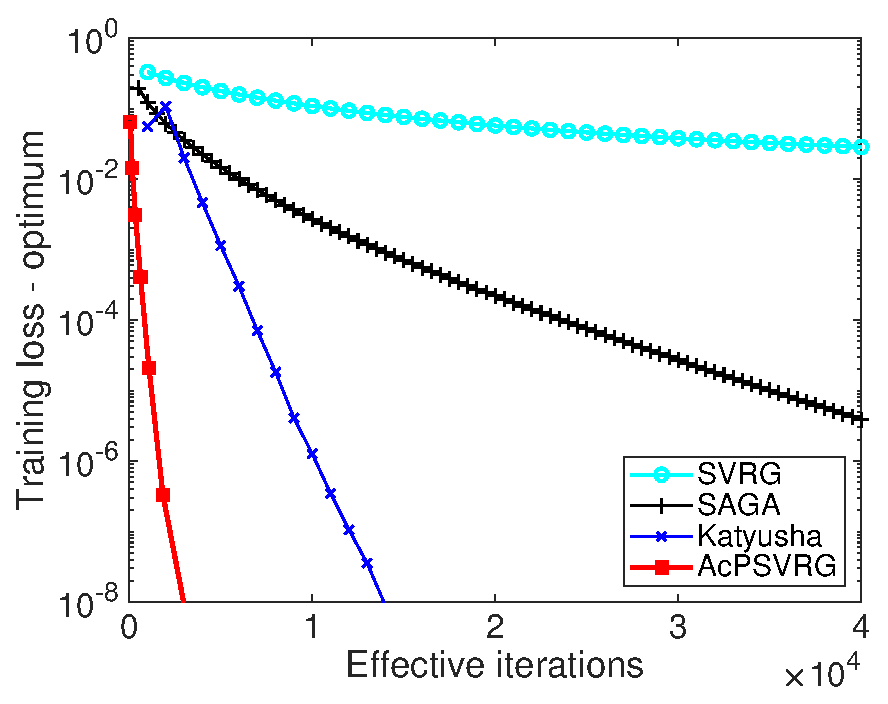
\includegraphics[width=0.24\linewidth]{Figures/real-sim_obj_dev_comparison_1worker.eps}}%
\subfigure[comparison on rcv1]{
\centering
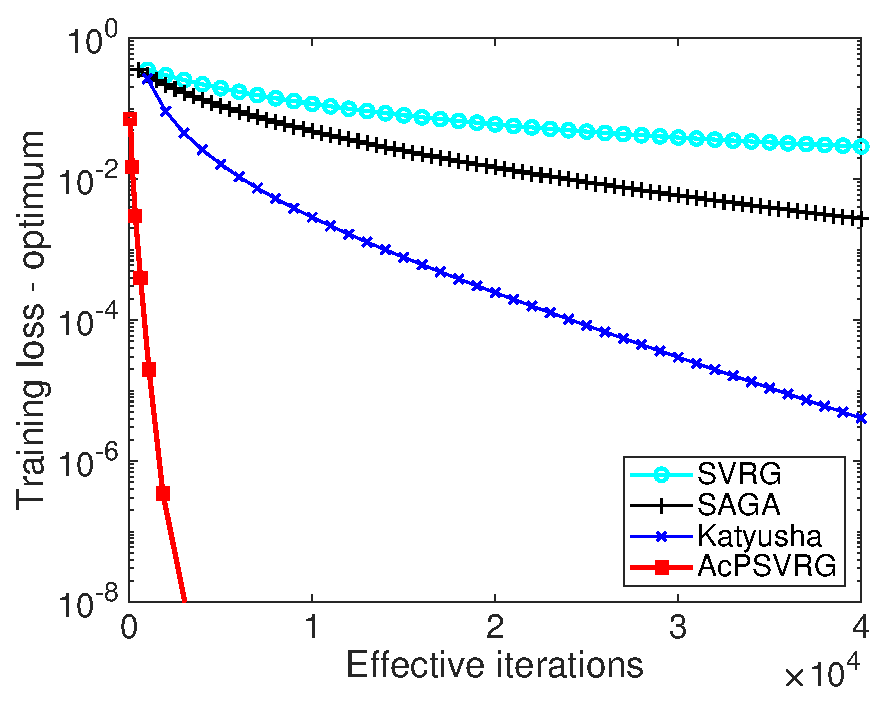
\includegraphics[width=0.24\linewidth]{Figures/rcv1_obj_dev_comparison_1worker.eps}}%
\setlength{\abovecaptionskip}{2pt}
\caption{Convergence performance of SVRG, SAGA, Katyusha, and AcPSVRG with single worker.}
\label{fig:AcPSVRG_seq}
\end{figure*}

\begin{figure*}[htbp]

\subfigure[comparison on ijcnn]{
\centering
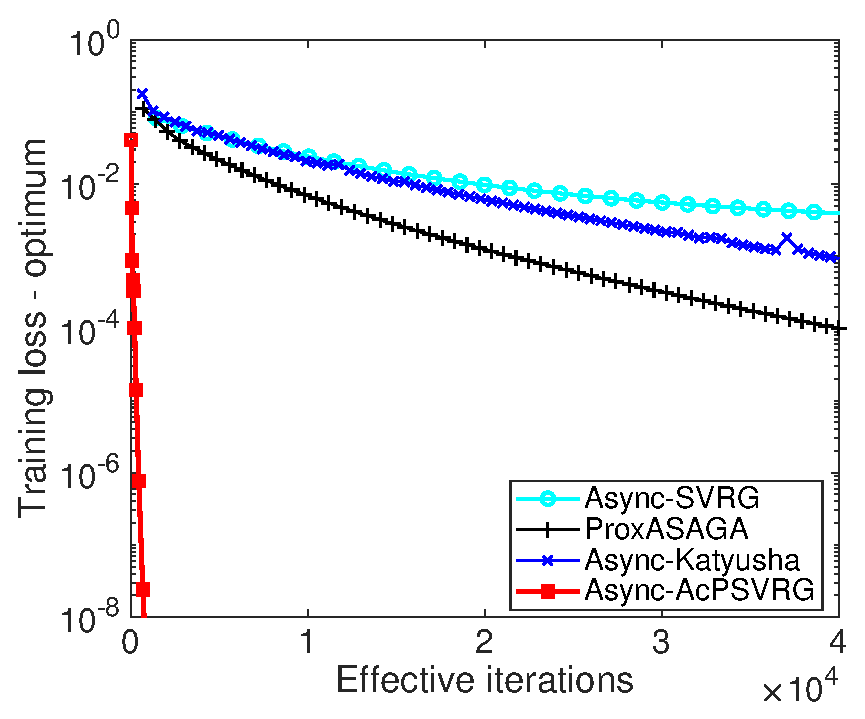
\includegraphics[width=0.24\linewidth]{Figures/ijcnn_obj_dev_comparison_16workers.eps}}%
\subfigure[comparison on covtype]{
\centering
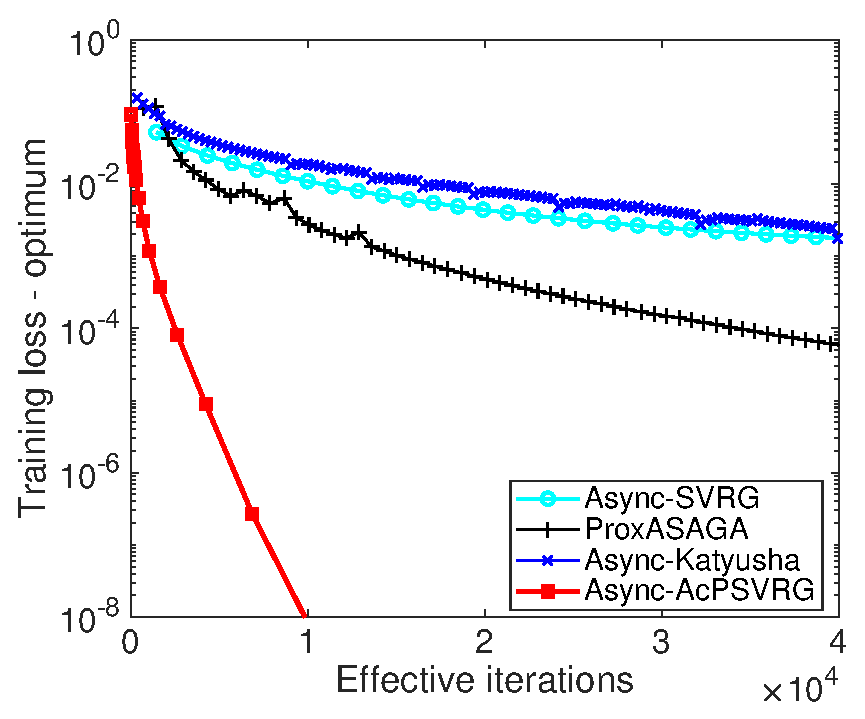
\includegraphics[width=0.24\linewidth]{Figures/covtype_obj_dev_comparison_16workers.eps}}%
\subfigure[comparison on real-sim]{
\centering
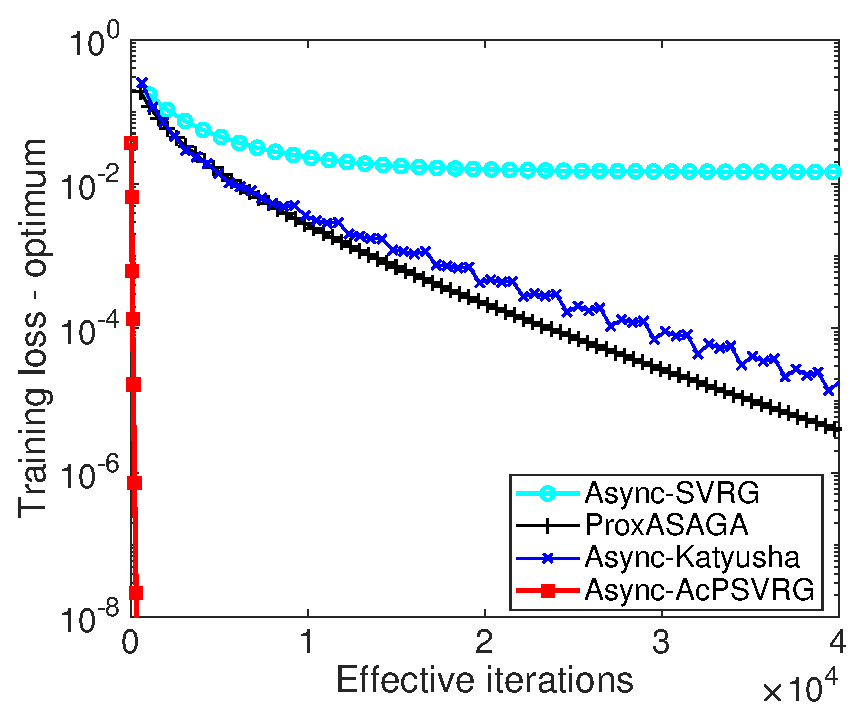
\includegraphics[width=0.24\linewidth]{Figures/real-sim_obj_dev_comparison_16workers.eps}}%
\subfigure[comparison on rcv1]{
\centering
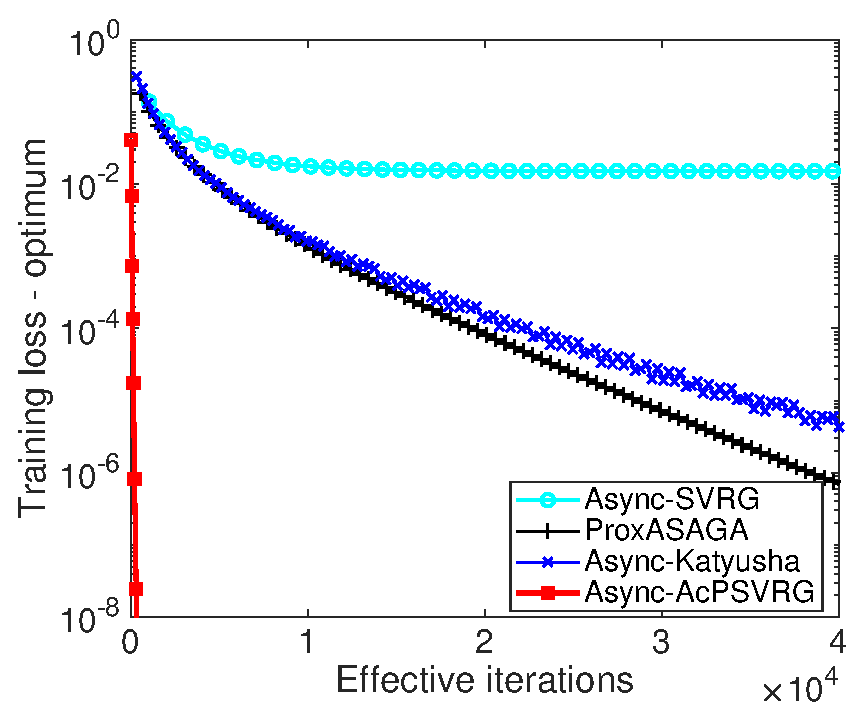
\includegraphics[width=0.24\linewidth]{Figures/rcv1_obj_dev_comparison_16workers.eps}}%

\subfigure[comparison on ijcnn]{
\centering
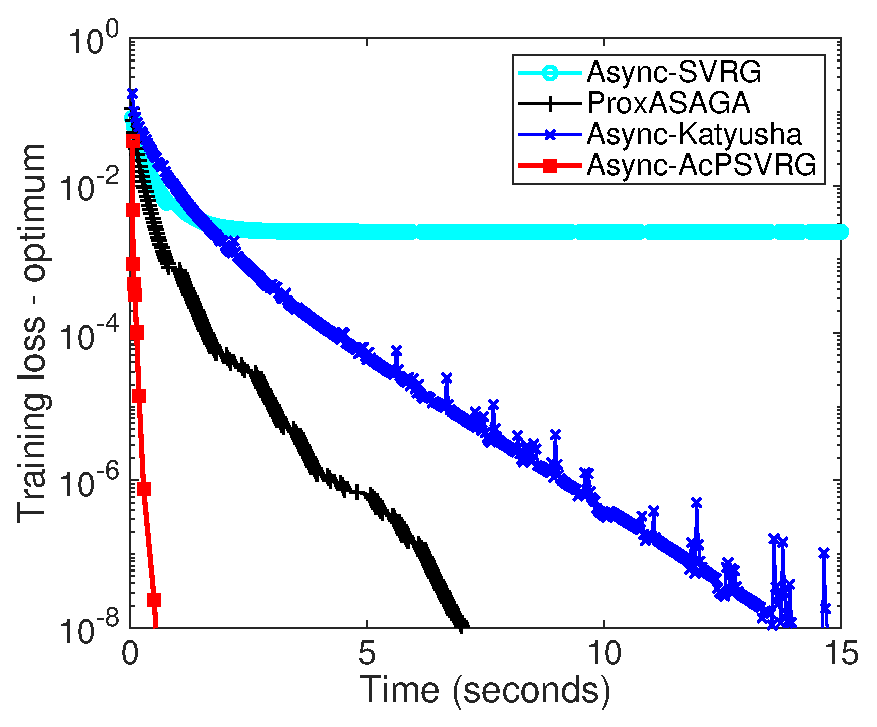
\includegraphics[width=0.24\linewidth]{Figures/ijcnn_obj_dev_comparison_time.eps}}%
\subfigure[comparison on covtype]{
\centering
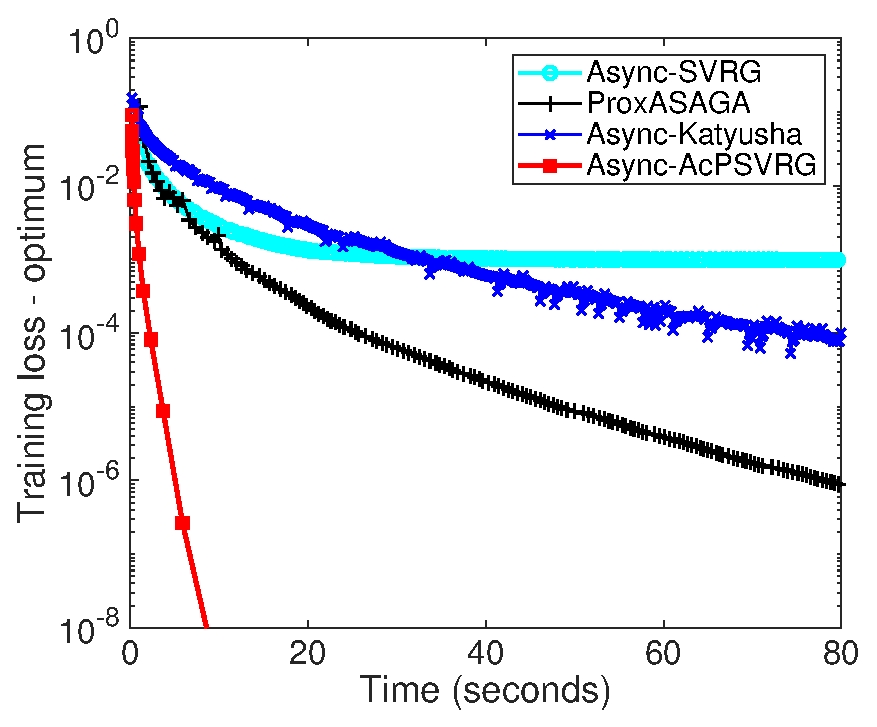
\includegraphics[width=0.24\linewidth]{Figures/covtype_obj_dev_comparison_time.eps}}%
\subfigure[comparison on real-sim]{
\centering
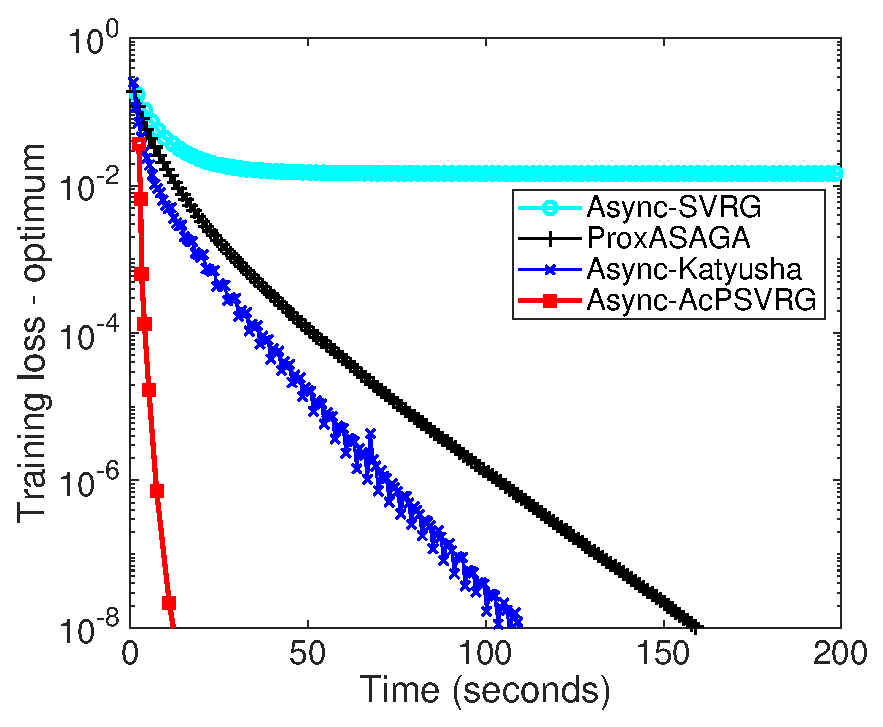
\includegraphics[width=0.24\linewidth]{Figures/real-sim_obj_dev_comparison_time.eps}}%
\subfigure[comparison on rcv1]{
\centering
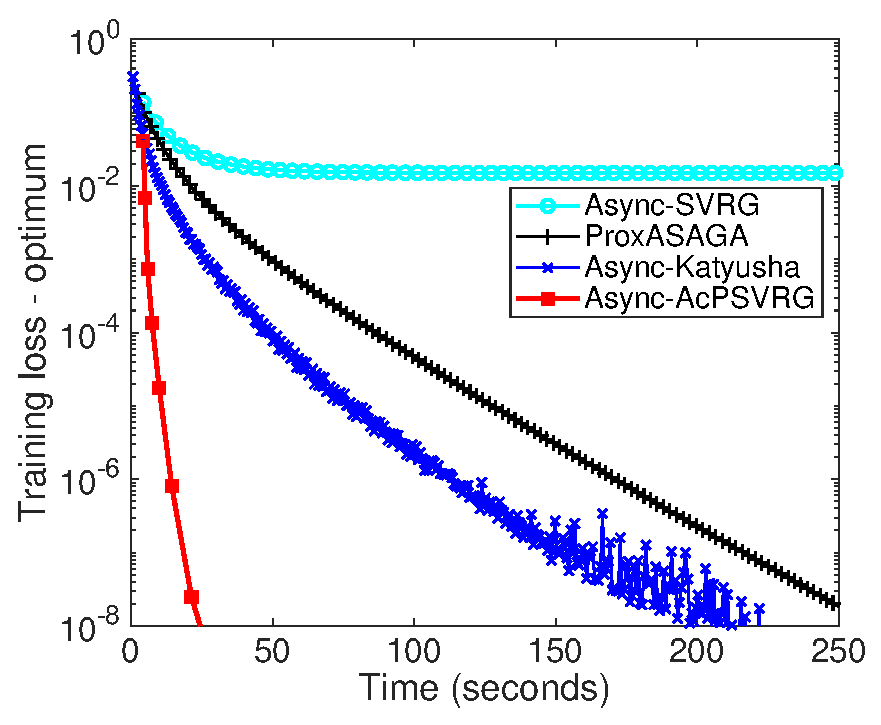
\includegraphics[width=0.24\linewidth]{Figures/rcv1_obj_dev_comparison_time.eps}}%
\setlength{\abovecaptionskip}{2pt}
\caption{Training loss residual $f(x) - f(x^*)$ versus iteration (top) and time (bottom) plot of Async-SVRG, ProxASAGA, Async-Katyusha, and Async-AcPSVRG. }
\label{fig:algo_comp}
\end{figure*}

For the second set of experiments we compare the performance of AcPSVRG with the variants of variance reduction stochastic gradient descent described earlier in this section.  
Figure \ref{fig:AcPSVRG_seq} shows the performance of AcPSVRG, SVRG, ProxASAGA and Katyusha with single worker. It is seen that the performance of AcPSVRG method outperforms other variants of SGD methods in all cases. We would like to verify in experiments if such benefits preserve for the asynchronous variants of these algorithms. We use 16 workers to compare the algorithms in this experiment. Figure \ref{fig:algo_comp} (top) shows the performance of asynchronous SVRG (Async-SVRG), ProxASAGA and asynchronous Katyusha (Async-Katyusha) regarding effective iterations on server which are similar to update steps in sequential setting. 
The performance gains are qualitatively similar to these algorithms on single worker in Figure \ref{fig:AcPSVRG_seq}. It is observed that Async-AcPSVRG always exhibits better convergence than other SGD variants. In particular, compared to Async-Katyusha, as a momentum acceleration method, Async-AcPSVRG shows significantly better convergence. Since the computation complexity of each epoch of these
algorithms is different, in Figure \ref{fig:algo_comp} (bottom) we directly plot the objective value versus the runtime for each of these algorithms. 
As seen in the figure, Async-AcPSVRG outperforms variance-reduced ProxSGD algorithms in all the cases. In particular compared to Async-Katyusha, as AcPSVRG uses only one auxiliary variable for calculation of momentum, it has lower complexity per iteration and so shows better convergence speed. 

Our proposed algorithms outperform Katyusha in several aspects. First, the plots of Async-Katyusha in asynchronous experiments show much more oscillations compared to our algorithms. This appearance
is caused by the sensitivity of Katyusha  to delayed gradients when calculating momentum terms with local partial data, which introduces variance in training process. Our algorithms do not show sensitivity on delayed gradients. Secondly, AcPSVRG needs to tune only one parameter for momentum acceleration for different datasets while Katyusha needs adjustment of two acceleration parameters in order to achieve a comparable level of performance.

\iffalse
\begin{table}
\begin{center}
\caption{Parameter setting for algorithm implementation. Lmax denotes Lipschitz constant, n is the number of data, and $\rho$ and  $m_s$ are specified to 1.25 and n/4. }
\begin{tabular}{ c|c|c|c } 
 \hline
 Algorithms & initial $\eta$ & Inner Loops & $\lambda$  \\ 
 \hline
 SVRG & 1/(10*Lmax) & 2n & 1e-4\\
 SAGA & 1/(10*Lmax) & n & 1e-4\\
 %SVRG++ & 1/(7*Lmax) & 2n \\ 
 %SVRG-Prox & 1/(7*Lmax) & 2n \\
 Katyusha & Lmax & 2n & 1e-4 \\
 AcPSVRG & 1.5/Lmax &  $\lceil{\rho\cdot m_s}\rceil$ & 1e-4\\
 \hline
\end{tabular}
\label{par_setting}
\end{center}
\end{table}
\fi









